% Chapter Template

\chapter{User studies} % Main chapter title

\label{Chapter6} % Change X to a consecutive number; for referencing this chapter elsewhere, use \ref{ChapterX}

\lhead{Chapter 6. \emph{User experience evaluation}} 
Human-Robot Interaction being a rapidly advancing area of research, there is a growing need for strong experimental designs and methods of evaluation. This will bring credibility and validity to scientific research that involves humans as subjects, as recognized in the psychology and social science fields. As robots are becoming more prevalent, accurate methods to assess how humans respond to robots, how they feel about their interactions with robots, and how they interpret the actions of robots are very important. Indriya platform being aimed at naive users it is very important to evaluate how people feel about the system. In this chapter, the experiment design process, data collection and analysis are discussed.

\section{Experiment protocol}
The interaction design process suggested in \cite{Rogers2011} has been followed. The main aspects of the experiment are as follows
\begin{itemize}
\item Identifying the participants: A set of participants were identified who have beginner to expert level programming skill to evaluate the platform
\item Relationship with participants: A professional relationship is maintained with the participants in order to reduce the bias in the evaluation process
\item Setting goals: The main goals of the experiment considered are
\begin{itemize}
\item Whether the participants understand the objective of the system?
\item Whether the participants able to use the system?
\item Whether the participants able to execute the designed scenario on the real robot?
\end{itemize}
\item Pilot studies: Before conducting the experiment with many participants, it has been decided to perform pilot studies on a small set of participants. This is to avoid ambiguities in the setup and data collection method that might arise when one directly conducts the real experiment.
\end{itemize}

For the pilot studies and also for the actual experiment, a handout describing the Indriya platform has been produced. The prepared handout is shown in Fig.~\ref{fig:handout}
\begin{figure}[H]
\centering
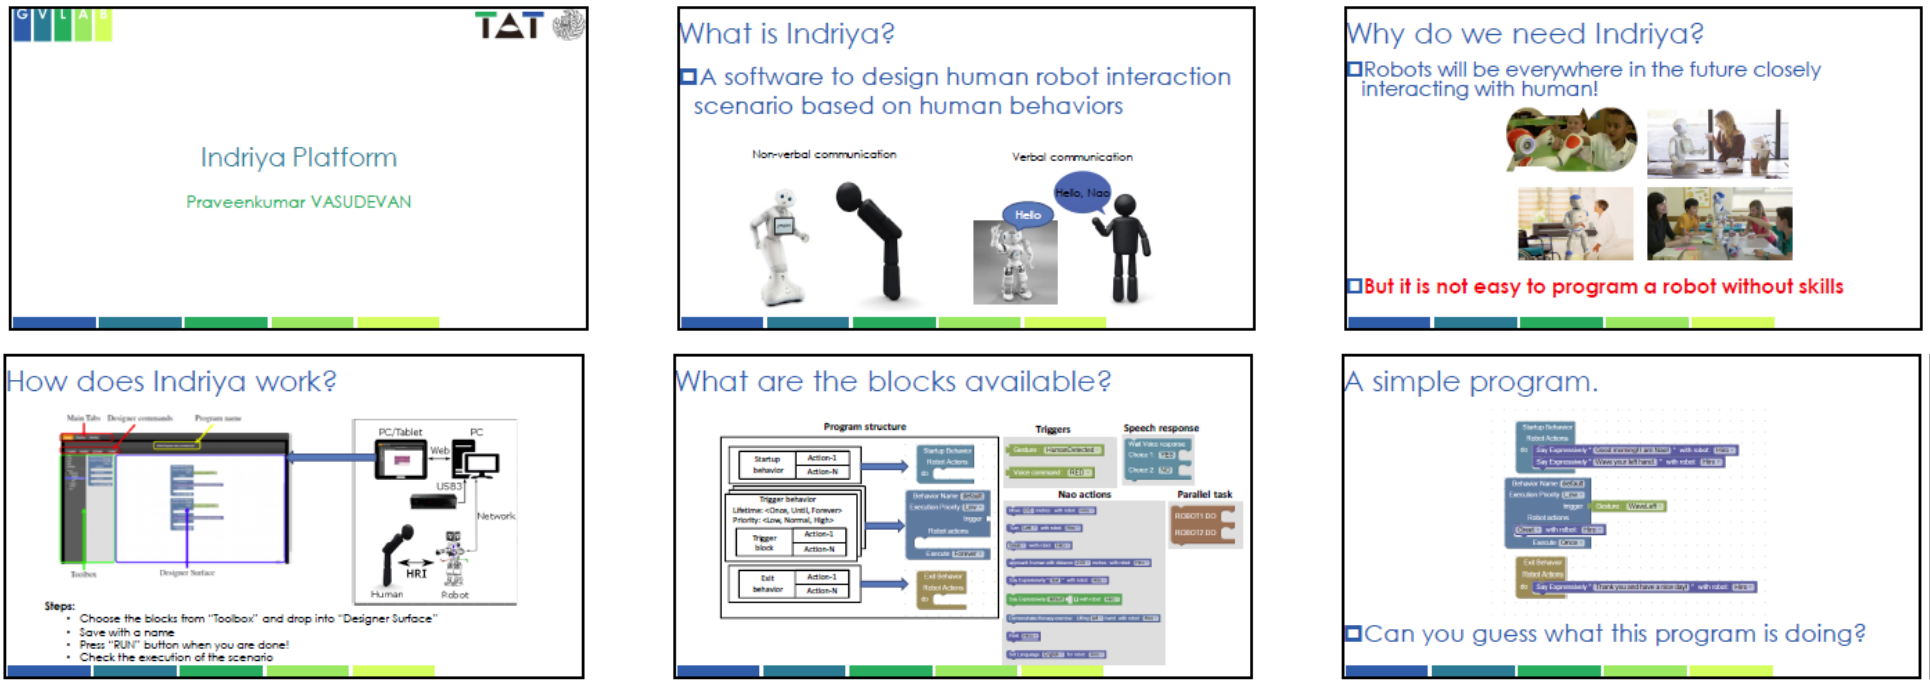
\includegraphics[width=\textwidth]{../thesis/assets/handout.png}
\caption[System description handout]{System description handout}
\label{fig:handout}
\end{figure}

The participants were given a short introduction about the system and were given a maximum of 90 minutes to think, design and execute the scenario designed. They were given a maximum of 2 chances to edit and execute the scenario on the real robot. Irrespective of whether they manage to complete what they desired at the end of two chances, they were asked to evaluate the system based on their experience of using the platform. Half of the participants were given an option to program two robots.

\section{Data collection method}
The self-assessment \cite{bethel2010review} technique has been used as the data collection method. A questionnaire has been framed in order to access various metrics of the user experience. The Google forms has been used to prepare the questionnaire. The questionnaire is at first made in English and after performing the pilot studies on a set of English speaking participants, it has been translated to Japanese with the help of a native Japanese speaker. The questionnaire has been integrated with the user interface. Soon after the participants design and execute the scenario, they could navigate to the \emph{Evaluate} screen (similar to the in-app rating system in modern applications) and evaluate the system. The Google forms integrated with user interface is shown in Fig.~\ref{fig:ui_evaluate}. 

\begin{figure}[H]
\centering
\begin{subfigure}[t]{0.48\textwidth}
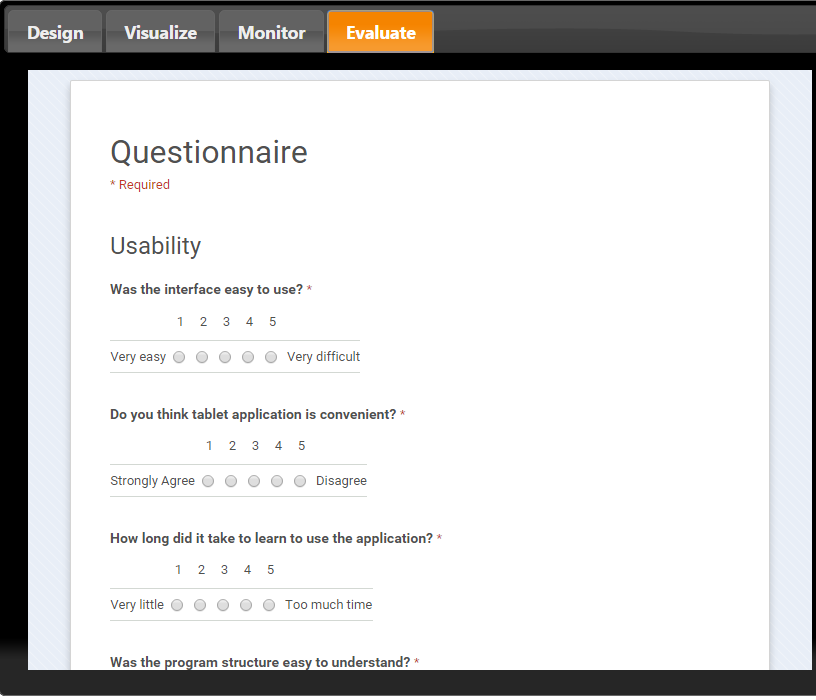
\includegraphics[width=\textwidth]{../thesis/assets/questionnaire_integration.png}
\caption[English]{English}
\label{fig:ui_evaluate_en}
\end{subfigure}
\begin{subfigure}[t]{0.48\textwidth}
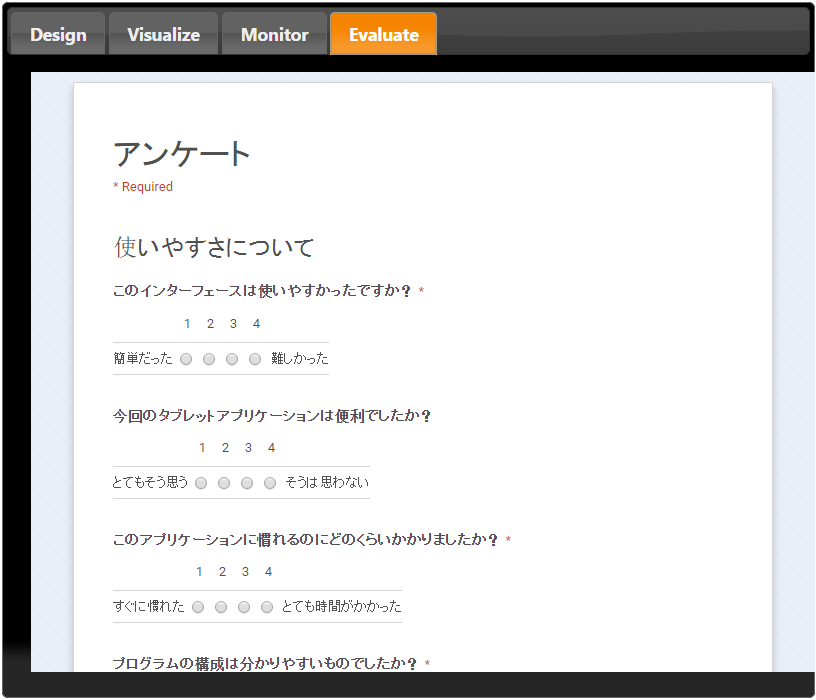
\includegraphics[width=\textwidth]{../thesis/assets/questionnaire_integration_jp.png}
\caption[Japanese]{Japanese}
\label{fig:ui_evaluate_jp}
\end{subfigure}
\caption[Questionnaire integration in UI]{Questionnaire integration in UI}
\label{fig:ui_evaluate}
\end{figure}

% \begin{figure}[H]
% \centering
% 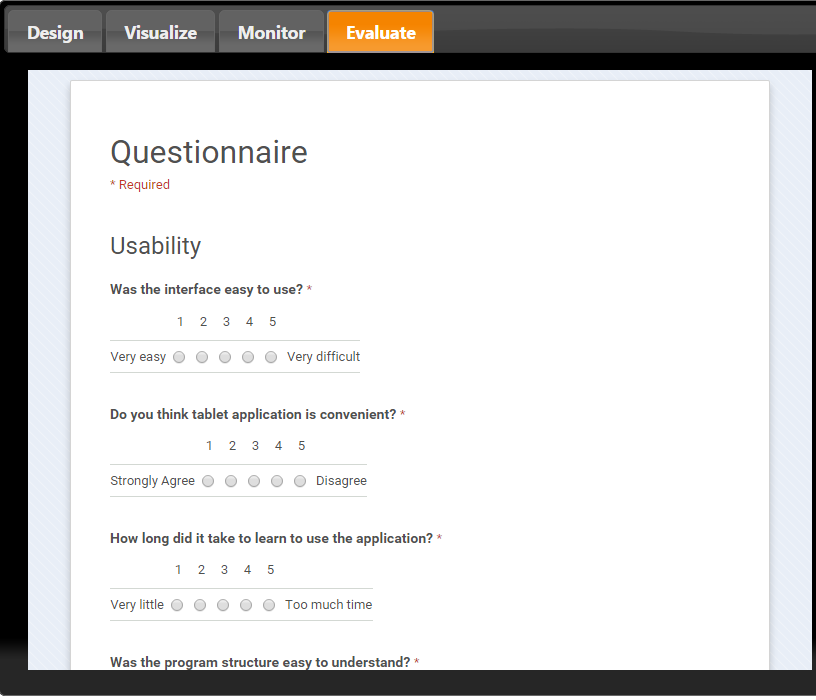
\includegraphics[width=0.7\textwidth]{../thesis/assets/questionnaire_integration.png}
% \caption[Questionnaire integration in UI]{Questionnaire integration in UI}
% \label{fig:ui_evaluate}
% \end{figure}

The questionnaire is presented in Appendix~\ref{AppendixD}. Most of the questions in the questionnaire are designed with a 4-point semantic differential scale and are designed in such a way that lesser the value better the user experience. The questionnaire has five sections namely
\begin{itemize}
\item Usability: To access the usability of the system
\item Execution: To access the performance of the system
\item System: To evaluate the overall capability of the system
\item Multi-robot programming: To access the usability of multi-robot programming
\item Background: To get an idea of the background of the users. However it is made sure that the sensitive information were not collected during the data collection.
\end{itemize}

\section{Data analysis}
Statistical analysis is performed on the data collected during the user study. Ten participants (Age mean: 22.3, SD: 4.47) were asked to program an interaction scenario using Indriya. About 50\% of the participants reported that they have beginner level proficiency in programming and do not have background in robotics. The usability metrics such as learnability, effectiveness, efficiency and satisfaction are focused on. To start with, \emph{Factor analysis} is performed on the data to find the dominant factors in the data. The mean and SD of the factor-wise usability metrics are shown in Fig.~\ref{fig:metrics}. Almost all the users found the system easy to learn to use and get started. About 80\% of the participants were able to create a scenario and execute it on real robot in less than 30 minutes.
 \begin{figure}
 \centering
 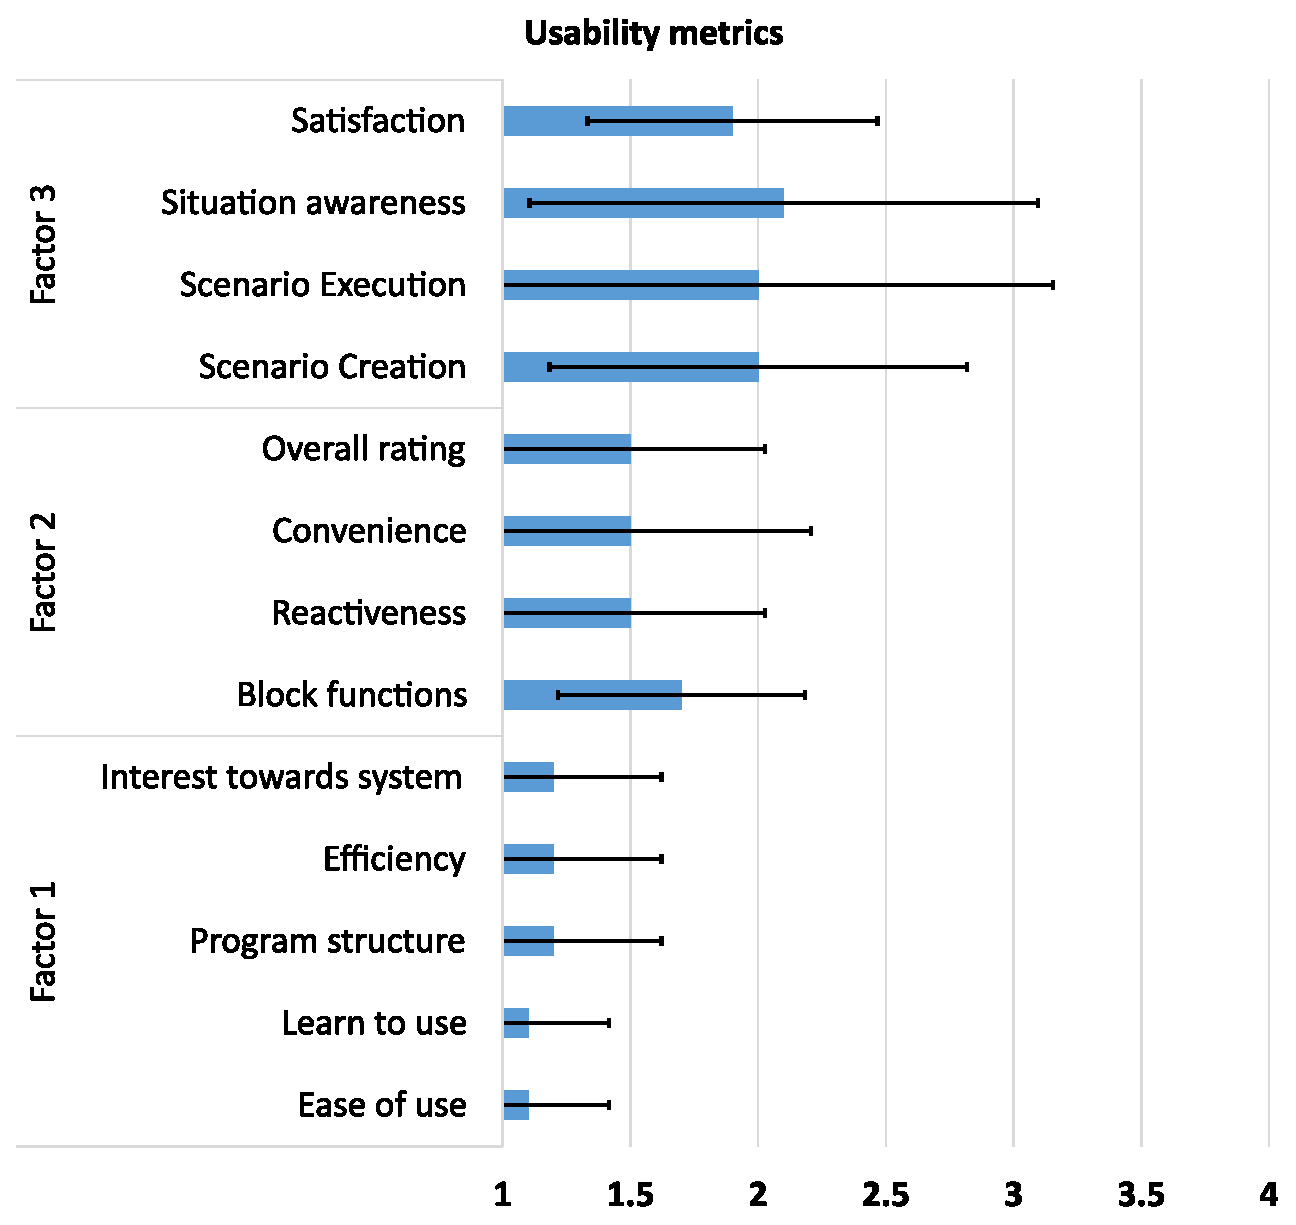
\includegraphics[width=\columnwidth]{../../thesis/assets/usability.eps}
 \caption[Usability metrics]{Usability metrics}
 \label{fig:metrics}
 \end{figure}

\begin{table}[h]
\caption{Pearson correlation coefficient}
\label{table:correlation}
\begin{center}
\begin{tabular}{|l|c|c|c|c|}
\hline
  {} & \textbf{Program}& \textbf{Scenario}& \textbf{Scenario}& \textbf{}\\
    {} & \textbf{structure}& \textbf{creation}& \textbf{execution}& \textbf{Reactiveness}\\
\hline
{} & {} & {} & {} & {}\\
\textbf{Learn to use} & {0.6667} & {-} & {-} & {-}\\
\hline
{} & {} & {} & {} & {}\\
\textbf{Convenience} & {-} & {0.7698} & {0.6804} & {-}\\
\hline
\textbf{Scenario}  & {} & {} & {} & {}\\
\textbf{creation}  & {-} & {-} & {0.7071} & {-}\\
\hline
\textbf{Scenario} & {} & {} & {} & {}\\
\textbf{execution} & {-} & {-} & {-} & {0.5477}\\
\hline
\end{tabular}
\end{center}
\end{table}
In order to find the correlation between various metrics shown in Fig.~\ref{fig:metrics}, Pearson correlation cofficient is computed. The most interesting outcomes are shown in Table~\ref{table:correlation}. As observed in the table, the users who found the program structure easy to understand also found the application easy to use. The users who felt that the application is convenient had a strong impact on the scenario creation. The users who were able to successfully execute the scenario rated that they found it easy to create the scenario and additionally found the robot reactive to gestures and voice commands which makes sense. 

\begin{table}
\centering
\small
\caption{Cronbach's $\alpha$}
\label{table:cronbach}
\begin{tabular}{|c|c|}
    \hline                             
    \textbf{Standardized} & \textbf{Unstandardized}\\
    \hline
     0.7302 & 0.8011 \\
    \hline
\end{tabular}
\end{table}

Furthermore, a statistic known as Cronbach's alpha (Table~\ref{table:cronbach}) reliability indicator is computed on the collected data. It measures the internal consistency reliability among a group of items that are combined to form a single scale \cite{bartneck2009measurement}. It reflects the homogeneity of the scale. Nunnally \cite{nunnally1978psychometry} recommends a minimum value of 0.7. As could be noticed from the table, the Cronbach's $\alpha$ is above 0.7, so we can conclude that the questionnaire used has sufficient internal consistency reliability.
 
\section{Summary and discussion}
Thanks to the user study, apart from evaluating the system, several extreme cases and the functionalities an user expects out of the system were determined. The summary of the observations are
\begin{itemize}
\item Speech recognition: Many users suggested the usage of an external microphone for the speech recognition. Most of the time during the interaction, the user is far away from the Kinect sensor so the voice recognition fails. This feedback from the user was immediately considered and an external microphone is used during the user study with the last four participants. 
\item Exit behavior: The interpretation of exit behavior was different from user to user. It was observed that the participants had difficulty in observing when the life time of all configured blocks complete.
\item Triggers: Many users attempted to aggregate multiple triggers together to fire the execution of a behavior block. Moreover some users wanted to fire a behavior block with some variable. The users also wanted to execute the trigger behavior blocks until a gesture trigger arrives or wait for a gesture (similar to voice response) to continue execution etc., These features will be considered to be implemented in the next version of the software.
\item Robot-robot interaction: The participants who programmed two robots went beyond human-robot interaction and tried to design robot-robot interaction scenarios. This possibility was not considered while authoring Indriya and it opens up new lines of research.
\end{itemize}